\section{Увод}

\subsection{Намена}
Овај документ представља спецификацију базе података за пројекат \textit{Gravity
Crusher}, на предмету Принципи софтверског инжењерства. У документу су дати IE модел
података, шема релационе базе података и детаљан опис табела и одговарајућих атрибута у
бази података. Овај документ представља основ за дизајн, имплементацију, интеграцију и
тестирање базе података и модула за комуникацију са базом података.

\subsection{Циљне групе}
Овај документ намењен је члановима развојног тима, који се воде спецификацијама наведеним
у документу приликом дизајнирања, имплементације, интеграције и тестирања овог
подсистема.

\subsection{Организација документа}
Остатак овог документа организован је у следећа поглавља:
    \begin{itemize}
        \item \textbf{Модел података} -- модел података у бази и шема релационе базе
                     података.
        \item \textbf{Табеле} -- опис табела унутар базе података.
    \end{itemize}

\subsection{Отворена питања}

\begin{table}[h!]
\centering

    \begin{tabu}{ || X[l] | X[l] | X[l] | X[l] || }
    \hline
    \textbf{Верзија} & \textbf{Датум} & \textbf{Кратак опис} & \textbf{Аутор} \\
    \hline
    \hline
    & & &\\
    \hline
    & & &\\
    \hline
    & & &\\
    \hline
    & & &\\
    \hline
    \end{tabu}
    \caption{Преглед отворених питања}
    \label{table:2}

\end{table}





\section{Модел података}

\subsection{IE нотација}

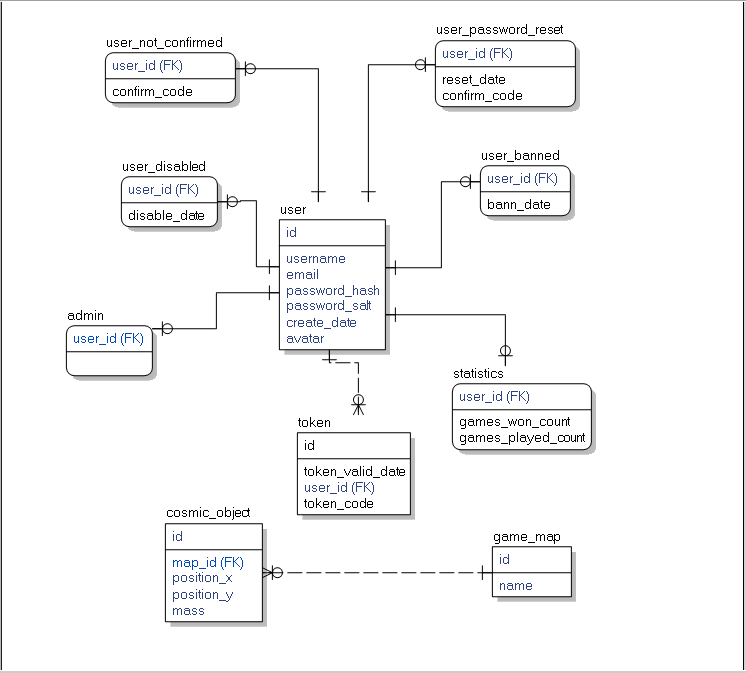
\includegraphics[width=\textwidth]{../resources/database-model.png}

\subsection{Шема релационе базе података}

\begin{enumerate}
    \item user(\underline{id}, username, email, password\_hash, password\_salt,
        create\_date)
    \item user\_banned(\underline{user\_id}, bann\_date)
    \item user\_disabled(\underline{user\_id}, disable\_date)
    \item user\_not\_confirmed(\underline{user\_id}, confirm\_code)
    \item user\_password\_reset(\underline{user\_id}, reset\_date, confirm\_code)
    \item token(\underline{id}, user\_id, token\_create\_date)
    \item statistics(\underline{user\_id}, games\_played\_count, games\_won\_count)
    \item game\_map(\underline{id}, name)
    \item cosmic\_object(\underline{id}, map\_id, position\_x, position\_y,
        velocity\_x, velocity\_y, mass)
\end{enumerate}



\section{Табеле}

\subsection{user}
Садржи основне податке о регистрованим корисницима апликације као и податке потребне за
пријављивање на кориснички налог.

\begin{table}[h!]
\centering
\small

    \begin{tabular}{ | m{0.45\textwidth} | m{0.22\textwidth} | m{0.1\textwidth} | m{0.1\textwidth} | }
    \hline
        \cellcolor{blue!25}\textbf{\textit{Name}} &

        \cellcolor{blue!25}\textbf{\textit{Datatype}} &
        \cellcolor{blue!25}\textbf{\textit{Is PK}} &
        \cellcolor{blue!25}\textbf{\textit{Is FK}} \\
    \hline
    \hline
        id & int(11) & Yes & No \\
    \hline
        username & varchar(25) & No & No \\
    \hline
        email & varchar(250) & No & No \\
    \hline
        password\_hash & varchar(128) & No & No \\
    \hline
        password\_salt & varchar(256) & No & No \\
    \hline
        create\_date & timestamp & No & No \\
    \hline
    \end{tabular}

\end{table}



\subsection{user\_not\_confirmed}
Садржи податке о томе који корисници су започели процес регистрације, али још увек нису потврдили
своје корисничке налоге путем e-mail верификације.

\begin{table}[h!]
\centering
\small

    \begin{tabular}{ | m{0.45\textwidth} | m{0.22\textwidth} | m{0.1\textwidth} | m{0.1\textwidth} | }
    \hline
        \cellcolor{blue!25}\textbf{\textit{Name}} &

        \cellcolor{blue!25}\textbf{\textit{Datatype}} &
        \cellcolor{blue!25}\textbf{\textit{Is PK}} &
        \cellcolor{blue!25}\textbf{\textit{Is FK}} \\
    \hline
    \hline
        user\_id & int(11) & Yes & Yes \\
    \hline
        confirm\_code & varchar(45) & No & No \\
    \hline
    \end{tabular}

\end{table}

\subsection{user\_password\_reset}
Садржи податке о томе који корсници су послали захтев за промену лозинке.

\begin{table}[h!]
\centering
\small

    \begin{tabular}{ | m{0.45\textwidth} | m{0.22\textwidth} | m{0.1\textwidth} | m{0.1\textwidth} | }
    \hline
        \cellcolor{blue!25}\textbf{\textit{Name}} &

        \cellcolor{blue!25}\textbf{\textit{Datatype}} &
        \cellcolor{blue!25}\textbf{\textit{Is PK}} &
        \cellcolor{blue!25}\textbf{\textit{Is FK}} \\
    \hline
    \hline
        user\_id & int(11) & Yes & Yes \\
    \hline
        reset\_date & timestamp & No & No \\
    \hline
        confirm\_code & varchar(45) & No & No \\
    \hline
    \end{tabular}

\end{table}

% Evil
\newpage

\subsection{user\_banned}
Садржи податке о корисницима којима је забрањено учествовање у игри.

\begin{table}[h!]
\centering
\small

    \begin{tabular}{ | m{0.45\textwidth} | m{0.22\textwidth} | m{0.1\textwidth} | m{0.1\textwidth} | }
    \hline
        \cellcolor{blue!25}\textbf{\textit{Name}} &

        \cellcolor{blue!25}\textbf{\textit{Datatype}} &
        \cellcolor{blue!25}\textbf{\textit{Is PK}} &
        \cellcolor{blue!25}\textbf{\textit{Is FK}} \\
    \hline
    \hline
        user\_id & int(11) & Yes & Yes \\
    \hline
        bann\_date & timestamp & No & No \\
    \hline
    \end{tabular}

\end{table}

\subsection{user\_disabled}
Садржи податке о корисницима који су деактивирали свој кориснички налог.

\begin{table}[h!]
\centering
\small

    \begin{tabular}{ | m{0.45\textwidth} | m{0.22\textwidth} | m{0.1\textwidth} | m{0.1\textwidth} | }
    \hline
        \cellcolor{blue!25}\textbf{\textit{Name}} &

        \cellcolor{blue!25}\textbf{\textit{Datatype}} &
        \cellcolor{blue!25}\textbf{\textit{Is PK}} &
        \cellcolor{blue!25}\textbf{\textit{Is FK}} \\
    \hline
    \hline
        user\_id & int(11) & Yes & Yes \\
    \hline
        disable\_date & timestamp & No & No \\
    \hline
    \end{tabular}

\end{table}

\subsection{token}
Садржи податке о тренутно коришћеним токенима.

\begin{table}[h!]
\centering
\small

    \begin{tabular}{ | m{0.45\textwidth} | m{0.22\textwidth} | m{0.1\textwidth} | m{0.1\textwidth} | }
    \hline
        \cellcolor{blue!25}\textbf{\textit{Name}} &

        \cellcolor{blue!25}\textbf{\textit{Datatype}} &
        \cellcolor{blue!25}\textbf{\textit{Is PK}} &
        \cellcolor{blue!25}\textbf{\textit{Is FK}} \\
    \hline
    \hline
        id\_token & int(11) & Yes & No \\
    \hline
        token\_create\_date & timestamp & No & No \\
    \hline
        user\_id & int(11) & No & Yes \\
    \hline
    \end{tabular}

\end{table}

\subsection{statistics}
Садржи статистичке податке за сваког корисника.

\begin{table}[h!]
\centering
\small

    \begin{tabular}{ | m{0.45\textwidth} | m{0.22\textwidth} | m{0.1\textwidth} | m{0.1\textwidth} | }
    \hline
        \cellcolor{blue!25}\textbf{\textit{Name}} &

        \cellcolor{blue!25}\textbf{\textit{Datatype}} &
        \cellcolor{blue!25}\textbf{\textit{Is PK}} &
        \cellcolor{blue!25}\textbf{\textit{Is FK}} \\
    \hline
    \hline
        user\_id & int(11) & Yes & Yes \\
    \hline
        games\_won\_count & int(11) & No & No \\
    \hline
        games\_playedn\_count & int(11) & No & No \\
    \hline
    \end{tabular}

\end{table}

% Evil
\newpage

\subsection{game\_map}
Садржи основне податке о мапама за игру.

\begin{table}[h!]
\centering
\small

    \begin{tabular}{ | m{0.45\textwidth} | m{0.22\textwidth} | m{0.1\textwidth} | m{0.1\textwidth} | }
    \hline
        \cellcolor{blue!25}\textbf{\textit{Name}} &

        \cellcolor{blue!25}\textbf{\textit{Datatype}} &
        \cellcolor{blue!25}\textbf{\textit{Is PK}} &
        \cellcolor{blue!25}\textbf{\textit{Is FK}} \\
    \hline
    \hline
        id & int(11) & Yes & No \\
    \hline
        name & varchar(45) & No & No \\
    \hline
    \end{tabular}

\end{table}

\subsection{cosmic\_object}
Садржи податке о космичким објектима који се налазе на некој од мапа за игру.

\begin{table}[h!]
\centering
\small

    \begin{tabular}{ | m{0.45\textwidth} | m{0.22\textwidth} | m{0.1\textwidth} | m{0.1\textwidth} | }
    \hline
        \cellcolor{blue!25}\textbf{\textit{Name}} &

        \cellcolor{blue!25}\textbf{\textit{Datatype}} &
        \cellcolor{blue!25}\textbf{\textit{Is PK}} &
        \cellcolor{blue!25}\textbf{\textit{Is FK}} \\
    \hline
    \hline
        id & int(11) & Yes & No \\
    \hline
        map\_id & int(11) & No & Yes \\
    \hline
        position\_x & float & No & No \\
    \hline
        position\_y & float & No & No \\
    \hline
        velocity\_x & float & No & No \\
    \hline
        velocity\_y & float & No & No \\
    \hline
        mass & float & No & No \\
    \hline
    \end{tabular}

\end{table}

